\documentclass[11pt, a4paper, USenglish]{article} % change ``USenglish'' to ``norsk'' if applicable.
\usepackage{subfig}
\usepackage{kyblab} % Contains all included packages. See kyblab.sty.
\usepackage{float}
\addbibresource{bibliography.bib} % Makes the bibliography file available to biblatex.

\begin{document}

% Titlepage
\title{LaTeX Lab Report Template}
\author{Group 53\\Adam Godtland Moumen\\Tobias De La Plaza Domaas\\Carl Joakim Duraj}
\date{20.11.2024}
\begin{titlepage}
    \maketitle
    \begin{figure}
    \centering
    
\includegraphics[width=0.5\textwidth]{figures/itk_ntnu}\\
    Department of Engineering Cybernetics
    \end{figure}
    \thispagestyle{empty}
\end{titlepage}

% Abstract
\newpage
\begin{abstract} 
%\addcontentsline{toc}{section}{Abstract} % add this if you want the abstract in the table of contents.
  This document outlines a few important aspects of a lab report. It contains some advice on both content and layout. The \LaTeX{} source for this document is also published, and you can use it as a template of sorts for your own report. You can find an up to date version of the source at \url{https://github.com/ntnu-itk/labreport}. The main file, ``labreport.tex'', defines the structure of the document. The ``preamble.tex'' file is the document preamble, and contains a lot of informative comments. The document is based on work done by Tor Aksel Heirung for TTK4135, and is now under continuous improvement by Andreas L. Fl{\aa}ten and Kristoffer Gryte (happily accepting suggestions and contributions from the community).

When you write your own report, this section (the abstract) should contain a \emph{very} short summary of what the lab is about and what you have done.
\end{abstract}
    
\thispagestyle{empty} % Avoid page numbering on the abstract page.

% TOC
\newpage
\tableofcontents
\thispagestyle{empty} % Avoid page numbering on the table of contents.

% Main content
\newpage
\setcounter{page}{1}
\section{Introduction}\label{sec:intro}
Your introduction should contain an overview of the work you were assigned, as well as a few sentences putting the work into a larger perspective. You should also give a quick description of how the report is organized (as is done below).

You should of course put most of the work into doing good work in the lab and then presenting it in the report. When presenting your work in the report, both content and presentation/layout matters. Since your only way of communicating your good effort in the lab is through writing about it here, the way you write about it is essential. This means that even if you have the very best controller but describe it poorly, you will probably not be rewarded for the good results. A plot showing perfect control is worth very little if it is not accompanied by a clear description of what it represents.

Layout is naturally less important than content, but it still matters. You can think of report writing like selling an apartment; when you present your apartment for potential buyers you will of course clean the apartment and make it good looking. How clean the apartment is does of course not determine its value, but it is still important since it influences the subjective value your buyers will put on the apartment. 

\subsection{Software}
You are of course free to use whatever software you want for report writing. You can also submit a handwritten report, although this is probably not a great idea if your handwriting can be hard to read. 

You can also use Word or a similar word processor. However, it is next to impossible to achieve decent layout with Word. The support for vector graphics (discussed later) is extremely poor, and text tends to look pretty bad (bad support for kerning and ligatures). Furthermore, math is both time consuming and difficult to input, and tends to look very ugly. In general, a report written in Word looks like a draft.

It is strongly recommended to use Latex. Unless you tweak the layout too much, your report will almost certainly look very good. Although it can take a bit of effort to get started, it is also much quicker to use than Word and similar programs. The support for math and vector graphics is also great.

If you are new to Latex, you can have a look at the source for this document to get started. You can also look at the presentation by~\cite{Berland2010} (in Norwegian) or consult~\cite{Oetiker2011}. Another good reason to learn Latex is that you probably don't want to write your master's thesis in something like Word, doing so would likely be very frustrating. Being reasonably fluent in Latex before you get that far will make your thesis work much smoother.

Some of you are probably fluent in Latex and might plan to write the report using it. Please resist the temptation (if any) to change the fonts, make super fancy headers (they are not necessary for a report like this), change the margins, change the paragraph indentation and/or spacing, and similar things.

A great tool for collaborating on Latex documents is ShareLaTeX at \url{https://www.sharelatex.com/}; if you use this you won't have to install anything on your computer. Texmaker at \url{http://www.xm1math.net/texmaker/} is a good cross-platform editor. Some people like Lyx, which is a Latex editor that behaves a little bit like Word. If you prefer to compile your Latex document on the command line, the latexmk \url{https://www.ctan.org/pkg/latexmk} command is a great tool included in most TeX distributions. There is also a simple Vim plugin that uses latexmk as its backend called LaTeX-BoX \url{https://github.com/LaTeX-Box-Team/LaTeX-Box}.

\subsection{Other Comments}
Unless you have a very good reason not to, you should write the report in English. If you have problems with Latex, the solution is usually just a few Google searches away.

This report is organized as follows: \Cref{sec:prob_descr} contains some course specific equations, and some tips on how to create illustrations. Several \LaTeX{} tips can be found in \Cref{sec:latex_tips}, such as how to create a table and matrix equations. \Cref{sec:figures} contains some advice on using plots from MATLAB\@. The closing remarks are in~\Cref{sec:conclusion}, respectively. \Cref{sec:matlab} contains a MATLAB file while \Cref{sec:simulink} shows an example Simulink diagram. The Bibliography can be found at the end, on page~\pageref{sec:bibliography}.

\section{Lab 1}
\subsection{Motivation}\label{sec:lab1_mot}
The motivation behind the first lab task was to create a PD regulator to the linearized
model of the helicopter \ref{eq:lin_model} for a cause to control its pitch. The equations
of motion can be find in \ref{eq:model_1}. For a simple visualization of the helicopter, see \ref{fig:helicopter_dia}.

\begin{subequations}\label{eq:model_1}
	\begin{align}
		\ddot{p}  &= -\frac{K_{f}l_{p}V_{d}}{J_{p}} = \frac{L_1Vd}{J_p} \label{eq:model_1_p} \\
		\ddot{e}  &= (2m_pgl_h-m_cgl_c)cos(e)+K_fl_hV_scos(p) = L_2cos(e)+L_3V_scos(p)\label{eq:model_1_e} \\
		\ddot{\lambda} &= \frac{l_hk_fV_scos(e)sin(p)}{J_{\lambda}} = L_4V_scos(e)sin(p) \label{eq:model_1_l} \\
	\end{align}
\end{subequations}

\subsection{Lab preperation}\label{sec:lab1_prep}
There were several tasks which needed to be done as preperation to the first lab day.
The first task was to derive the equations of motion from a given diagram of the helicopter \ref{fig:helicopter_dia}.
This task required thoroughly analyzing the forces which the helicopter is affected by.
When this was done, it was needed to linearize the model around the equlibrium (all system states equal zero) represented by \ref{fig:helicopter_dia} such that 
creating controllers would be easier. We were now ready to implement a PD controller given by \ref{eq:PD}
and insert this into the linearized equation of pitch acceleration, to control the pitch to a given reference.
The last preperation for lab 1 was to make a test plan for pole placements to the pitch control. We used the equations in \ref{eq:pole_place}.

\begin{subequations}\label{eq:lin_model}
	\begin{align}
        \tilde{V_d} &= V_d-V_{d,origo} = V_d\\
        \tilde{V_s} &= V_s-V_{s,origo} = V_s+\frac{L_2}{L_3}\\
		\ddot{p}  &= \frac{L_1\tilde{V_d}}{J_p} = K_1V_d\label{eq:lin_p} \\
		\ddot{e}  &= \frac{L_3\tilde{V_s}}{J_e} = K_2\tilde{V_s}\label{eq:lin_e} \\
		\ddot{\lambda} &= \frac{L_4L_2\tilde{p}}{L_3J_{\lambda}} = K_3p\label{eq:lin_l} \\
	\end{align}
\end{subequations}
\begin{subequations}\label{eq:PD}
	\begin{align}
        V_d &= K_{pp}(pc-p)-K_{pd}\dot{p}
	\end{align}
\end{subequations}
\begin{subequations}\label{eq:pole_place}
	\begin{align}
    K_{pd} &= -\frac{s_2+s_1}{K_1}\\
    K_{pp} &= \frac{s_2s_1}{K_1}
	\end{align}
\end{subequations}

\subsection{Hypotheses/Test plan}
We wanted to expirement the controller by setting the poles at several different positions, including real and complex numbers.
We prepared twelve different tests, with hyoptheses coming from control theory which as for poles in LHS of s plane are exponentially stable, RHS are unstable and poles in origo are stable.
The table \ref{tab:testskjema_lab1} gives an overview of our tests and their s-values, stability result and hypotheses.
During the tests we have a step equal 10V in the disturbance of the system from 15s to 15.2s. We also added a step in the elevation reference equal -0.55 until 5 seconds have past.
\begin{table}[h]
\centering
\phantomsection % Creates an anchor for the hyperlink
 % Place the label at the top of the table
    \begin{tabular}{||c c c c c||} 
     \hline
     Test & Poles & Pitch ref & Hypotheses & Result \\ [0.5ex] 
     \hline\hline
     1 & -1,-1 & 0 & Exp. Stability & Exp. Stability \\ 
     \hline
     2 & -5,-5 & 0 & Exp. Stability & Exp. Stability \\
     \hline
     3 & $-1\pm j5$  & 0 & Exp. Stability & Exp. Stability  \\
     \hline
     4 & $-1\pm j$ & 0 & Exp. Stability & Exp. Stability \\
     \hline
     5 & $-5\pm j$ & 0 & Exp. Stability & Exp. Stability \\  
     \hline
     6 & $-5\pm j5$ & 0 & Exp. Stability & Exp. Stability \\ 
     \hline
     7 & $\pm j$ & 0 & Marginal Stability & Unstable \\  
     \hline
     8 & $\pm j5$ & 0 & Marginal Stability & Unstable \\ 
     \hline
     9 & $0$ & 0 & Marginal Stability & Unstable \\ 
     \hline
     10 & $1\pm j$ & 0 & Unstable & Unstable \\ 
     \hline
     11 & -1,1 & 0 & Unstable & Unstable \\ 
     \hline
     12 & 1,1 & 0 & Unstable & Unstable \\ [1ex]
     \hline
    \end{tabular}
    \caption{Test scheme}
    \label{tab:testskjema_lab1}
\end{table}
\subsection{Results}
We have decided to plot results of only five of the done tests, such that the plots are not redundant.
The plot \ref{fig:pitch_plot} visualize a time series for test 1,4,7,9 and 11. Y-axis is the pitch measured in radians. X-axis shows each timestep. The reason behind this is to include different pole-values which
with also different specific hypotheses and result. For all tests the reference of the pitch was at 0 rad. The step functions in elevation reference and disturbance are specifically visible for test 1 and test 4. 
At around 5 seconds the pitch seems to be affected by the elevation going to 0, and the pitch has even bigger response to the step in disturbance at 15 seconds. The controller manages to send the pitch back around zero 
fairly fast and smooth. 

When looking at plot \ref{fig:pitch_plot} test 9 and test 11 is cut off early. The reason behind this is that 
the pitch became so unstable, where at a point it could provide harm to the helicopter. As safety measure we cut its power early. 
Test 1 and 4 have a similar run, which is expected as they both have same real part. However even though test 4 have an imaginary part, 
it dosent seem to add more swings than the one without an imaginary part.

\begin{figure}[h!]
    \centering
    \subfloat[Plots from test 1 and 4]{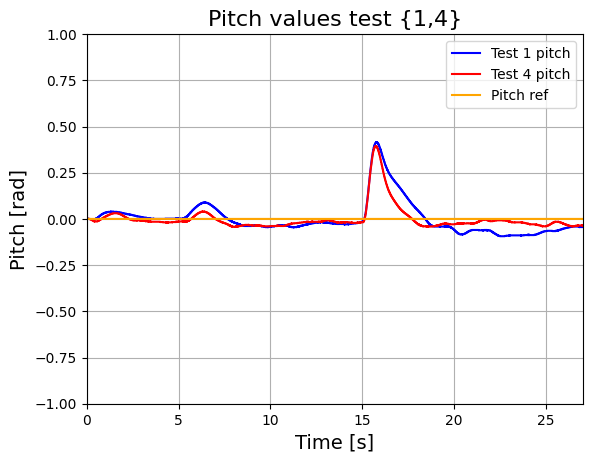
\includegraphics[width=0.5\textwidth]{figures/lab1pitchV1.png}}\hfill
    \subfloat[Plots from test 7,9 and 11]{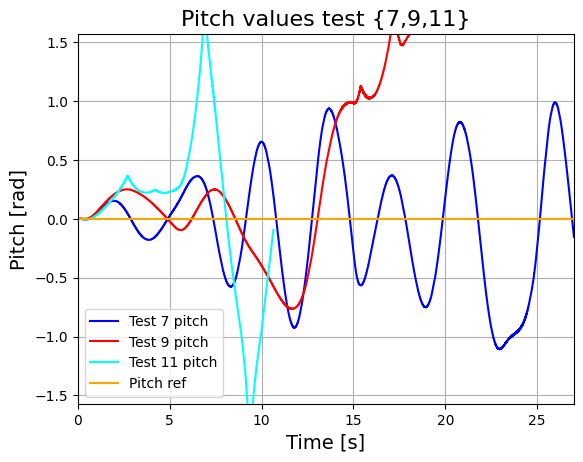
\includegraphics[width=0.5\textwidth]{figures/lab1pitchV2.png}}
    \caption{Timeseries of pitch angle in [rad].}
    \label{fig:pitch_plot}
\end{figure}     

\subsection{Conclusion}
The results match our hypotheses for the tests well. Poles in left hand side of the s plane give exp. stability and poles in right hand side give unstability. However if the real parts of the poles were close to the 
imaginary axis, the closed loop system became unstable. This is likely a result of the real system being heavily unlinear, 
and us working with a simple linearized model of it, leaving several margins of error. Sadly when saving data from the lab day we didnt accompany time series of the controller output, which would be a valuable asset to discuss in this report. 
It would be interesting to visualize and compare values the PD controller generated throughout the tests.  


\section{Conclusion}\label{sec:conclusion}
This does not have to be long, but try to write a few reasonable closing remarks.

\addcontentsline{toc}{section}{Appendix} % Remove this if you don't want the appendix included in the table of contents.
\appendix

\section{MATLAB Code}\label{sec:matlab}
This section should contain your MATLAB code. DO NOT attach files posted online (that you didn't write). Note that the method used to input code below does not look as pretty when the lines are too long.

\subsection{plot\_constraint.m}\label{sec:plot_constraint_m}
\lstinputlisting{code/plot_constraint.m}\section{Simulink Diagrams}\label{sec:simulink}
This section should contain your Simulink diagrams. Just like the plots, these should be in vector format, like in \Cref{fig:simulink}. Make them tidy enough to understand.

\subsection{A Simulink Diagram}
\Cref{fig:simulink} shows a Simulink diagram. You can use the \texttt{print\_simulink.m} function, included in the source code repository for this document, to export a Simulink model to EPS\@.
\begin{figure}[htb]
	\centering
		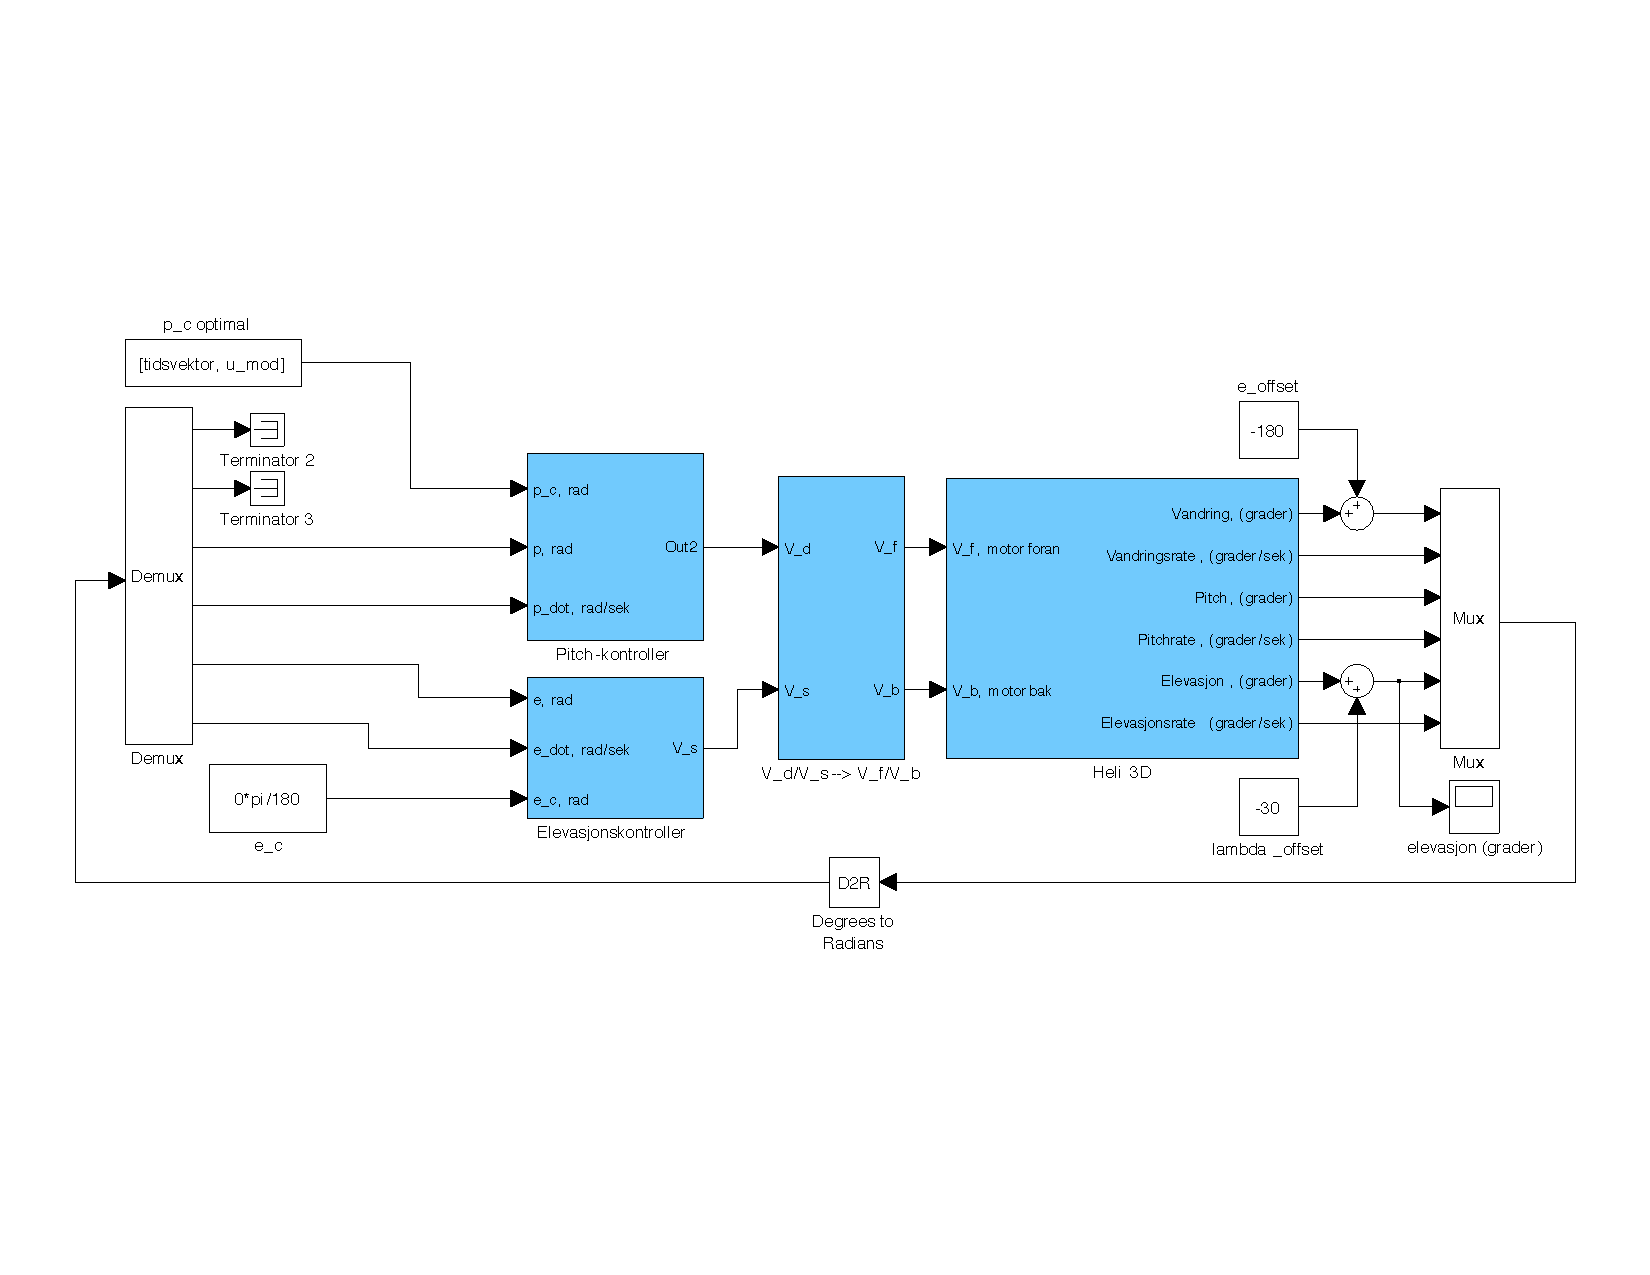
\includegraphics[width = \textwidth]{figures/simulink.pdf}
	\caption{A Simulink diagram.}
\label{fig:simulink}
\end{figure}

% \input simply inserts the contents of the file, while \include forces a \newpage.
% See \input vs. \include: http://tex.stackexchange.com/questions/246/when-should-i-use-input-vs-include

% References
\newpage
\addcontentsline{toc}{section}{References}
\printbibliography{}
\label{sec:bibliography}

\end{document}
